\chapter{Super-Kamiokande Detector Calibration}
\label{chp:superkcalib}


In order to achieve optimal event reconstruction for physics analyses, calibration of the Super-Kamiokande detector is crucial. For example, when constructing Monte Carlo simulations of certain processes in the detector, facets of the experiment such as properties of the water, photomultiplier tube response and the inner detector and outer detector electronics are all calibrated so that input parameters for the Monte Carlo simulations can be obtained. This chapter will concern itself with the inner and outer detector calibration, including photomultiplier tube and electronics calibration, PMT gain calibration, quantum efficiency determination and hit timing and charge information calibration. 

\subsection{Inner detector calibration}


\subsubsection{High-voltage setting calibration}

The high-voltage (HV) setting for all photomultiplier tubes need to adjusted individually so all the PMTs produce the same amount of charge for a certain light intensity recieved by them. Placing a light source which distributes light isotropically in the centre of the inner detetector to achieve this calibration means that there is no position in the detector from which the inner detector PMTs are equidistant, so each PMT will not recieve the same amount of light from the light source. To avoid this problem, a set of 420 pre-calibrated PMTs inside the detector were used, seperated into groups relating to their geometrical distance from the HV calibration light source (see Figure \ref{fig:hvcalib} for their location with respect to the other photomultiplier tubes.)

\begin{figure}
    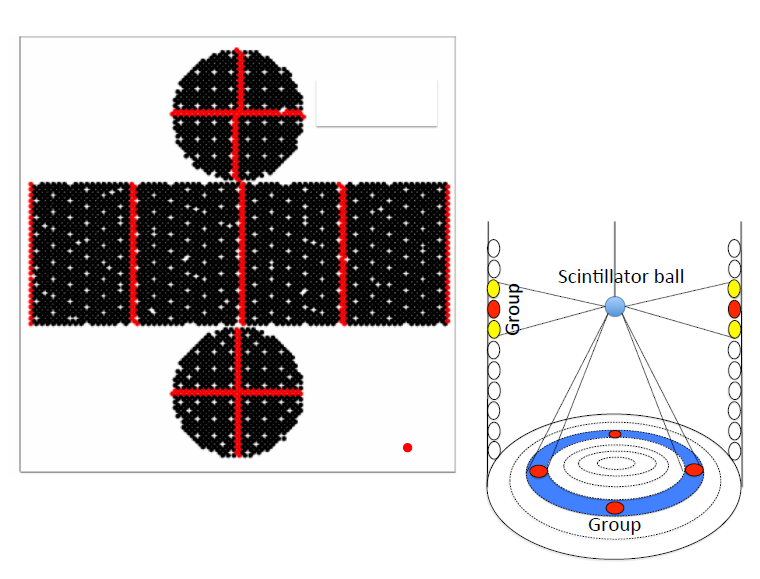
\includegraphics[width=\textwidth]{Figures/hvcalib.png}
\caption{Location of 420 reference PMTs used for HV setting calibration. The red lines in show the placement of these PMTs with repsect to the others (left). The grouping of these PMTs due to their geometry in relation to the light source is also shown (right) }
    \label{fig:hvcalib}
\end{figure}




\subsubsection{Relative gain calibration}

Understanding the timing information from the hit photomultiplier tubes depends on how well the charge from the hit PMT is calculated. To conceive charge calibration, a quantity called photomultiplier tube ''gain" must be calculated. ''Gain" is the conversion factor from the number of photoelectrons produced by the hit PMT and charge, and calibration of this quantity is what interpretation of very high energy events (TeV scale) rely on. Quantum efficiency is another quantity used for the calibration of low energy physics events (such as detection of solar neutrinos), due to them consisting of single photoelectron (single-pe) hits: it is the ratio of the number of the number of photoelectrons emitted by the cathode to the number of photons that are incident on the photomultiplier tube window. Quantum efficiency is particularly useful for low energy events because the number of photons arriving at the photomultiplier tube window is small. Super-Kamiokande calibration converts this measure of quantum efficiency into ''QE" by multiplying the quantum efficiency by the collection efficiency of the photoelectrons onto the first dynode inside the PMT \ref{abeCalibrationSuperKamiokandeDetector2014}. Knowing the gain and QE of each PMT in the detector is important in order to accurately measure the output charge from each individual PMT, which is done by first calculating the relative gain gain difference among all PMTs and then work out the average gain difference over all PMTs in the detector. After this, the variation away from this average gain value can be calculated for each seperate inner detector photomultiplier tube, and the gain value for each can be extracted. 

The relative gain difference is calculated by two measurements using a light source to produce constant-intensity flashes. The first measurement involves using the light source to produce high-intensity flashes so that all photomultiplier tubes in the detctor gets a certain number of photons, and the second measurement has the light source produce low-intensity flashes so that only a few PMTs are hit. teh first measurement provides an average charge value ($Q_{o b s}(i)$) for each inner detector PMT, while the second measurement gives single photoelectron hits, providing a number of times ($N_{o b s}(i)$) that a single PMT gives a charge which is greater than the PMT threshold value. Equation \ref{eq:gaineq} shows how these two values are calculated from the the high and low intensity flash values ($I$), the acceptance of the PMT(i) ($a(i)$), the QE value of the PMT ($\varepsilon_{q e}$) and the PMT gain $G$. 

\begin{align}
Q_{o b s}(i) \quad \propto \quad I_{high} \times a(i) \times \varepsilon_{q e}(i) \times G(i) \\
N_{o b s}(i) \quad \propto \quad I_{low} \times a(i) \times \varepsilon_{q e}(i)
\end{align}
\label{eq:gaineq}

Therefore, by simply dividing these two values of $Q_{o b s}(i)$ and ($N_{o b s}(i)$) the average gain over all PMTs can be calculated.  Figure \ref{fig:relativegain} shows the spread of the relative gain over all the PMTs. 

\begin{figure}
    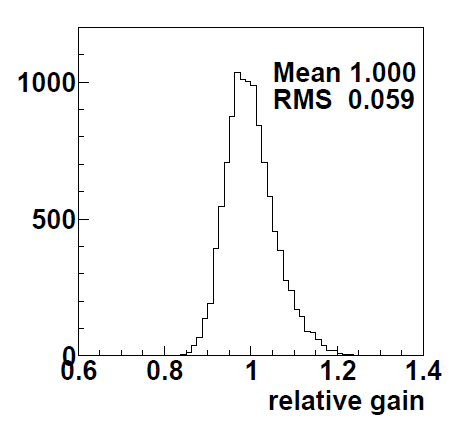
\includegraphics[width=\textwidth]{Figures/relativegain.png}
\caption{Relative gain of PMTs in Super-Kamiokande}
    \label{fig:relativegain}
\end{figure}

\subsubsection{Absolute gain calibration}

In order to calculate absolute gain, the single photoelectron distrubution needs to be measured, this is because absolute gain relates to the observed charge in the photomultplier tube with the number of photoelectrons produced. A nickel source (which includes a Californium-252 which decays to provides a source of neutrons) emits gamma rays in an isotropic distribution after neutron capture. This nickel source is placed in the centre of the inner detector and the gamma rays produced are detetced by all the inner detector PMTs. On average the observed number of photoelectrons is 0.004 per event per PMT, meaning that single p.e. hits are observed for more than 99\% of the hits. The observed charge distribution of all the hits from this nickel source is used to give the average charge, which is used as a conversion factor from a charge measurement in picoColoumbs and single photo-electrons. The factor is 2.658pC per photoelectron (calculated at the beginning of SK-IV) which is then used to extract the single-p.e. distribution, shown in Figure \ref{fig:singlepe}.

\begin{figure}
    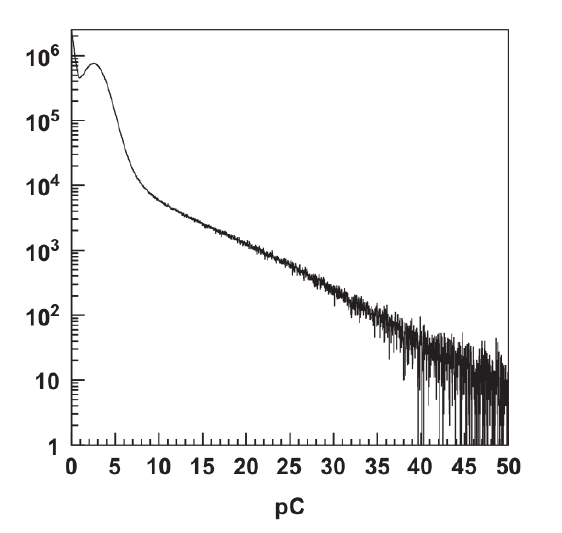
\includegraphics[width=\textwidth]{Figures/singlepe.png}
\caption{Single p.e distribution of charge in pC }
    \label{fig:singlepe}
\end{figure}



\subsubsection{Relative quantum efficiency measurement}

To measure the relative quantum efficiency, the gamma rays from neutron capture on the nickel source are simulated. Inside this simulation, a common value of QE is used for all the ID PMTs to predict the number of hits for each PMT. Comparing this number of hits to the actual data obtained for each individual PMT by calculating the ratio between them provides us with a value for relative QE for each inner detetor PMT which is then used inside the simulation. 

\subsubsection{Timing information calibration}


